\chapter{Evaluation Metrics}\label{ch:evaluation-metrics}
In this chapter, I will define metrics used for performance evaluation.

Before doing so, it is necessary to describe constituents of the confusion matrix~\ref{fig:confusionmat}.

\begin{figure}[H]
    \centering
    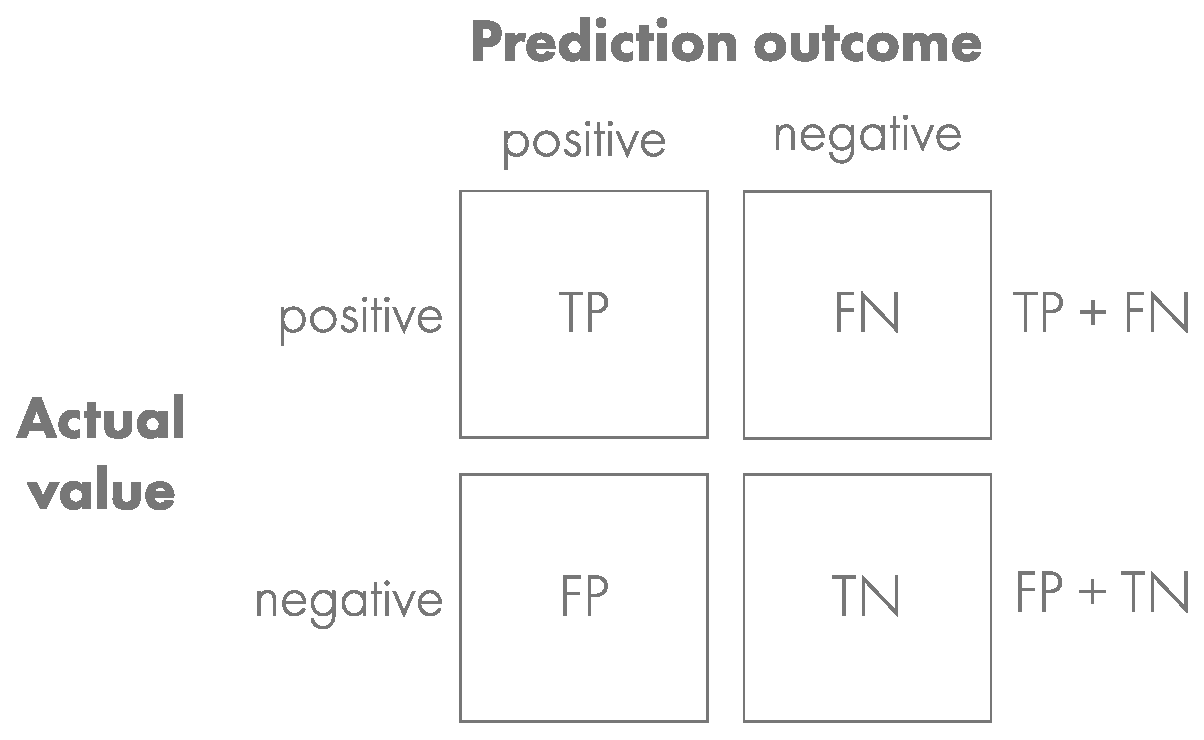
\includegraphics[width=0.9\columnwidth]{images/implementation/confusion_matrix.eps}
    \caption{Confusion matrix~\cite{ConfMat}}
    \label{fig:confusionmat}
\end{figure}

\textbf{True Positives} (TP) is the number of actual positives being predicted as positive.

\textbf{False Positives} (FP), also known as \textbf{type I error}, is the number of actual negatives being predicted
as positive.

\textbf{False Negatives} (FN) is the number of actual positives being predicted as negative.
FN is called \textbf{type II error}.

\textbf{True Negatives} (TP) is the number of actual negatives being predicted as negative.

With these terms introduced, we can proceed with a definition of precision~\ref{sec:precision} and
recall~\ref{sec:recall}.

\section{Precision}\label{sec:precision}
Precision~\cite{PreRec} is the number of relevant instances among the retrieved instances.
Mathematically speaking, precision is defined as the following fraction:
\begin{equation}
    Precision = \frac{TP}{TP + FP},
\end{equation}
where TP and FP are the constituents of the confusion matrix~\ref{fig:confusionmat}.

A useful feature of precision is that it can be used to detect faulty model and dataset mislabelings.
This property was extensively used during system implementation~\ref{ch:implementation}.

\section{Recall}\label{sec:recall}
Recall~\cite{PreRec} (also called sensitivity) is the fraction of the total amount of relevant instances that were
actually retrieved.
A definition of recall is the following:
\begin{equation}
    Recall = \frac{TP}{TP + FN},
\end{equation}
TP and FN were described in the beginning of the chapter.

\section{$F_1$-score}\label{sec:f-score}
$F_1$-score is the harmonic mean of precision and recall.
The metric is defined by the following formula:
\begin{equation}
    F_1 = 2 \cdot \frac{precision \cdot recall}{precision + recall}.
\end{equation}

The important property of this metric is that it successfully deals with skewed data.
This scenario occurs when there is much more positives than negatives in the data or vice versa.
A typical example is a classifier used to diagnose a rare illness.
If the model always predicted false, the accuracy\footnote{Sum of true positives divided by the number of predictions.}
would be high even though the system would be essentially useless.